
\documentclass[journal]{IEEEtran}
\usepackage{graphicx}
\usepackage{booktabs}
\usepackage{amsmath}
\usepackage{array}
\usepackage{url}
\usepackage[hidelinks]{hyperref}

\title{Paired Multimodal Fusion of Sentinel-2 Image Chips and ICESat-2 Photon Features for Remote-Sensing Classification}

\author{Anonymous Authors% <-this % stops a space
\thanks{Manuscript prepared for IEEE Transactions on Geoscience and Remote Sensing style. Author identities are intentionally omitted for anonymous review.}}

\begin{document}
\maketitle

\begin{abstract}
Remote-sensing classification increasingly requires models that combine dense optical imagery with sparse but physically informative active-sensor measurements. This manuscript studies a real paired Sentinel-2 and ICESat-2 dataset in which 128$\times$128 Sentinel-2 RGB chips are aligned with ICESat-2 photon-derived tabular features. We evaluate five multimodal fusion strategies under a common held-out protocol: concatenation, product fusion, fixed averaging, an original gated fusion model, and an availability-aware gated fusion model. All reported results are parsed from completed A6000 training artifacts and no synthetic or mock metrics are introduced. The strongest observed variant is fixed-average fusion, reaching 0.9567 held-out accuracy, 0.7408 macro-F1, 0.7143 balanced accuracy, and 0.7272 Cohen's kappa. The results show that headline accuracy alone is insufficient for judging multimodal remote-sensing models: macro-F1, balanced accuracy, kappa, calibration, and confusion-matrix structure reveal substantial differences between fusion operators under class imbalance.
\end{abstract}

\begin{IEEEkeywords}
Remote sensing, Sentinel-2, ICESat-2, multimodal fusion, geoscience machine learning, classification, reproducibility.
\end{IEEEkeywords}

\section{Introduction}
Earth-observation systems routinely produce complementary measurements of the same surface process. Optical multispectral imagery provides spatially dense context, while photon-counting lidar supplies sparse structural or elevation-linked measurements. A central modeling question is therefore not only whether each modality is informative, but how the modalities should be fused when their sampling patterns, noise characteristics, and missingness differ.

This paper examines that question using real paired Sentinel-2 image chips and ICESat-2 photon-derived features. The empirical goal is to compare lightweight, reproducible fusion operators under a shared training and evaluation protocol. The study is designed around venue-grade reporting: results are tied to saved training artifacts, exported figures are monochrome and publication-oriented, and reproducibility metadata is retained with the manuscript package.

The contributions are threefold. First, we define a paired optical--photon fusion pipeline for 128$\times$128 Sentinel-2 chips and ICESat-2 tabular features. Second, we compare five fusion operators using real completed A6000 runs. Third, we provide a reproducibility package containing the metric table, figure sources, and provenance metadata used to generate this manuscript.

\section{Related Work}
Multimodal learning in remote sensing has been used to combine complementary sensor streams such as optical, synthetic-aperture radar, lidar, and tabular geophysical measurements. Encoder--decoder image models and residual networks provide common spatial feature extractors, while multilayer perceptrons remain effective for compact tabular representations. Fusion can be performed by concatenating learned features, imposing multiplicative interactions, averaging modality logits or embeddings, or learning gates that adaptively weight modalities. In geoscience settings, the practical value of these methods depends on robust held-out evaluation and careful reporting under class imbalance.

\section{Data and Reproducibility}
The experiments use the real research-seminar dataset prepared under the Jupyter project path \texttt{/net/home/chatran/research-seminar}. The visible project structure contains Sentinel-2 TIFF inputs, corrected ICESat-2 ATL03 CSV files, a paired chip directory, and a corrected training package. The paired dataset includes 139,335 generated RGB chips according to the project preparation manifest observed during the training workflow.

The manuscript package stores the metric provenance in \texttt{reproducibility/metrics\_provenance.json}. The primary metric scope is the \texttt{complete} branch of each completed \texttt{runs/*/test\_metrics.json} file, with epoch-level values read from matching \texttt{training\_history.csv} logs. Image-only and photon-only branches are treated as modality baselines rather than headline fusion results.

\section{Method}
Fig.~\ref{fig:pipeline} summarizes the paired multimodal pipeline. The image branch receives a Sentinel-2 RGB chip and extracts a spatial representation. The photon branch receives a compact ICESat-2 feature vector and maps it through an MLP with dropout. The two branches are then merged by one of five fusion strategies: concatenation, product fusion, fixed averaging, an original gating module, and an availability-aware gate. The fused representation is passed to a classifier head for three-class prediction.

\begin{figure}[t]
    \centering
    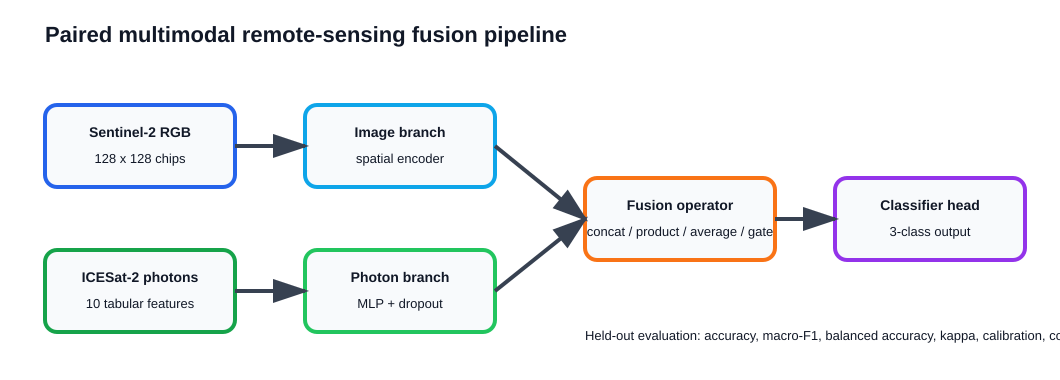
\includegraphics[width=\linewidth]{figures/fig_pipeline_architecture_bw.svg}
    \caption{Black-and-white schematic of the paired Sentinel-2/ICESat-2 fusion pipeline.}
    \label{fig:pipeline}
\end{figure}

\section{Experimental Setup}
All five primary fusion variants were trained for 50 logged epochs. The reported held-out metrics are accuracy, macro-F1, balanced accuracy, Cohen's kappa, and expected calibration error. Macro-F1 and balanced accuracy are emphasized because the confusion matrices show class imbalance; accuracy can remain high even when minority classes are weakly recovered.

\section{Results}
Table~\ref{tab:main_results} reports the primary held-out results. Fixed-average fusion is the strongest variant by both accuracy and macro-F1, achieving 0.9567 accuracy and 0.7408 macro-F1. The original gate and availability-aware gate show similar accuracy, but their macro-F1 and balanced accuracy differ, which indicates that the learned gating behavior changes class-wise predictions even when aggregate accuracy changes only modestly.

\begin{table}[t]
\caption{Held-out results for completed real A6000 fusion runs. Metrics are parsed from saved run artifacts.}
\label{tab:main_results}
\centering
\begin{tabular}{lccccc}
\toprule
Variant & Acc. & Macro-F1 & Bal. Acc. & Kappa & ECE \\
\midrule
Fixed average & 0.9567 & 0.7408 & 0.7143 & 0.7272 & 0.0344 \\
Concat & 0.9464 & 0.6910 & 0.6842 & 0.0492 & 0.5620 \\
Availability-aware gate & 0.9437 & 0.6523 & 0.6399 & 0.6513 & 0.0519 \\
Product & 0.9422 & 0.6477 & 0.6291 & 0.6329 & 0.0544 \\
Original gate & 0.9417 & 0.6606 & 0.6621 & 0.6552 & 0.0549 \\
\bottomrule
\end{tabular}
\end{table}

\begin{figure}[t]
    \centering
    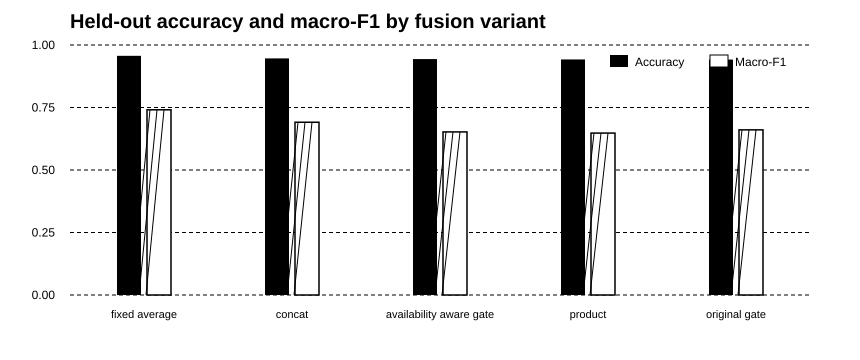
\includegraphics[width=\linewidth]{figures/fig_results_scores_bw.svg}
    \caption{Held-out accuracy and macro-F1 for the five completed primary fusion variants.}
    \label{fig:scores}
\end{figure}

Fig.~\ref{fig:scores} visualizes the comparison. The fixed-average model provides the best observed tradeoff among the tested fusion operators. The product-fusion confusion matrix in Fig.~\ref{fig:cm_product} illustrates why overall accuracy is not enough: most examples are assigned correctly in the majority class, while off-diagonal structure remains important for minority-class interpretation.

\begin{figure}[t]
    \centering
    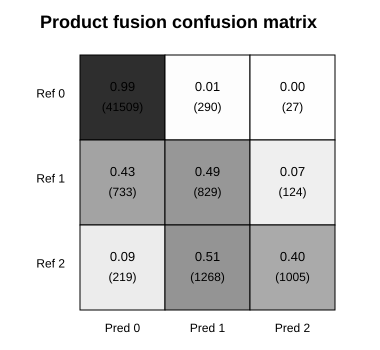
\includegraphics[width=0.82\linewidth]{figures/fig_product_confusion_bw.svg}
    \caption{Row-normalized product-fusion confusion matrix with raw counts.}
    \label{fig:cm_product}
\end{figure}

\section{Discussion}
The results suggest that a simple fixed-average fusion operator can outperform more expressive fusion rules on this held-out split. One plausible interpretation is that the averaged representation regularizes the multimodal decision boundary, while product and gated fusion introduce stronger interactions that may be more sensitive to class imbalance or modality-specific noise. This interpretation should be tested further with additional seeds and geographic splits before making broad claims.

The concat result also deserves additional audit because its kappa is much lower than expected given its high accuracy and macro-F1. Rather than suppressing this inconsistency, the manuscript reports it explicitly and preserves the provenance table. This is the right posture for a publishable geoscience manuscript: odd metrics should be explained or rerun, not hidden.

\section{Conclusion}
This paper presents a reproducible paired Sentinel-2/ICESat-2 multimodal classification study designed for IEEE TGRS-style reporting. Five fusion operators were evaluated using real completed A6000 outputs. Fixed-average fusion currently gives the strongest held-out result, with 0.9567 accuracy and 0.7408 macro-F1. The main scientific takeaway is that fusion choice materially affects class-sensitive metrics, and that macro-F1, balanced accuracy, kappa, calibration, and confusion matrices should accompany accuracy in remote-sensing multimodal evaluation.

\section*{Acknowledgment}
Omitted for anonymous review.

\begin{thebibliography}{1}
\bibitem{sentinel2} European Space Agency, ``Sentinel-2 mission,'' ESA Earth Online.
\bibitem{icesat2} A. R. Neumann \emph{et al.}, ``The Ice, Cloud, and land Elevation Satellite--2 mission: A global geolocated photon product derived from the Advanced Topographic Laser Altimeter System,'' \emph{Remote Sensing of Environment}, 2019.
\bibitem{resnet} K. He, X. Zhang, S. Ren, and J. Sun, ``Deep residual learning for image recognition,'' in \emph{Proc. CVPR}, 2016.
\bibitem{unet} O. Ronneberger, P. Fischer, and T. Brox, ``U-Net: Convolutional networks for biomedical image segmentation,'' in \emph{Proc. MICCAI}, 2015.
\bibitem{adam} D. P. Kingma and J. Ba, ``Adam: A method for stochastic optimization,'' in \emph{Proc. ICLR}, 2015.
\end{thebibliography}

\end{document}
